% !TEX root = BioInspired.tex

\chapter{Evolutionary Algorithms - Text Chapter 3}

\section{Problem 3.1 and 3.2}
Implement the various hill-climbing procedures and the simulated annealing algorithm to solve the problem exemplified in Section 3.3.3. use a real-valued representation scheme for the candidtate solutions (variable x). By comparing the performance of the algorithms, what can you conclude?

For 3.2, also implement an genetic algorithm to do the same.

For the simple hill climbing, try different initial configurations as attempts at finding the global optimum. Was this algorithm succesful?

Discuss the sensitivity of the algorithms in relations to their input parameters.

\subsection{Problem Information}

The goal of the problem in 3.3.3 referenced by the text was to find the global maximum of the equation $g(x) = 2^{-2(\frac{x-.1}{.9})^2}sin(5\pi x)^6$. By inspection of the graph given in the textbook, we know that the optimal x value is 0.1, and the global maximum is 1. All algorithms were evaluated by whether or not they reliably converged to this answer.

\subsection{Deterministic Hill Climb}

\subsubsection{Algorithm Description}
The first algorithm we implemented was the deterministic hill climb. In this program, we chose a random starting x value, and input a fixed number of time-steps. At each time-step, the algorithm checks to the left and right of the current position by a fixed step-size. If a better solution is found, the algorithm moves one step in that direction. This repeats until no improvement can be made, or the maximum number of iterations is reached.

\subsubsection{Algorithm Performance}
This algorithm, in general, was not succesful. Even when the starting domain was restricted between -1 and 1, the algorithm only converged to the global maximumin  approximately 10\% of the trials. In the other 90\% of the trials, the starting x value was outside the "hill" of the global maximum, and it would converge to to a local maximum instead.

\subsubsection{Sensitivity}
We considered the sensitiviy of the algorithm to 3 input parameters: starting x value, step size, and number of time steps.

This method is extremely sensitive to the starting x value. If there is not a monotonicaly increasing slope from the starting value to the global maximum, deterministic hill climb will not find it. This algorithm does, however, always find the nearest local maximum, and does so very quickly.

The resolution of the final result depends on the step size, but as long as the step size is reasonably small it does not effect whether or not the algorithm will converge on a local maximum.

The final result is sensitive to the maximum number of iterations. If the distance between the starting x value and the x value of the local maximum is greater than the number of iterations multiplied by the step-size, the local maximum will not be reached when the program terminates.

\subsection{Stochastic Hill Climb}

\subsubsection{Algorithm Description}
The stochastic hill climb was a slight variation on the deterministic hill climb. Instead of looking left and right by a fixed step size, we instead would pick a random floating point number from a uniform distribution between -p and p, where p was one of our input parameters. At each time step, we would generate this random number and add it to the current x value. If the new location had a higher fitness than the old location, we would replace the current x value with that new x value. This algorithm terminated once the maximum number of iterations was reached, or if the fitness of the current x value was equal to the global maximum, which we knew to be 1 by examination of the graph of the function.

\subsubsection{Algorithm Performance}
This algorithm was hit and miss and highly sensitive to paramters, as will be discussed in the next section. In general, this algorithm performed better than the deterministic hill climb because it had the potential to jump out of local maxima. However, it also had the potential to jump away from the global maximum rather than converging.

For this particular problem, we were able to find a set of parameters that nearly always converged to the global maximum in the time allowed, but from a computational perspective, it wasn't much better than random search.

\subsubsection{Sensitivity}
We analyzed three input parameters: starting x value, perturbation size - referred to as p above, and maximum number of iterations.

The starting x value had some impact on whether the algorithm would converge, but not nearly as much as in the deterministic version because the algorithm had the potential to jump out of local maxima in favor of maxima with higher fitness. Of course, if the starting x value was randomly generated very close to the global maximum, it nearly guaranteed the algorithm would converge to the global maximum.

The most important parameter was the perturbation size. A very large perturbation allowed the algorithm to jump out of local maxima much more frequently, but it also took much longer to converge to any maxima, and may not converge at all if the maximum number of iterations was too small. If the perturbation size was very small, the algorithm would quickly converge on a maxima, but be unable to jump out of local maxima. The proper value for this parameter seems to be highly problem dependant, and is affected by the maximum allowable number of iterations. If an infinite number of iterations were allowed, having a very large perturbation size would be allowable. The algorithm may jump between maxima with a high frequency, but the algorithm never chooses a new x value with a lower fitness than the current one, so it would eventually find the global maximum.

The maximum number of iterations on its own had little effect on the final solution except in the case noted in the discussion about perturbation size.

\subsection{Shotgun Hill Climb}

\subsubsection{Algorithm Description}

This algorithm is also known as iterated hill climb in the text, but we liked the Wikipedia name a little better. The basic premise of shotgun hill climb is to run a hill  climb algorithm many times with different starting positions, and keep track of the best of all runs. For this particular problem, we chose to iteratively apply the stochastic hill climbing method. Since the stochastic hill climb nearly always converged, applying it with many different starting x values basically guaranteed convergence. In our application, we chose the starting x value randomly for each iteration, but another method would be to uniformly sample the feature space.

\subsubsection{Algorithm Performance}

This algorithm worked very well. For this problem, it might be the fastest and most reliable solution. However, for problems with very large and complex feature spaces, fully sampling the space might not be desirable or even possible. At the very least it is an easy first attempt for finding a least a very good local maximum of a complex feature space.

\subsubsection{Sensitivity}

The most interesting feature of the shotgun hill climb is its insensitivity to starting parameters. Even if the hill climb algorithm were set up with poor starting conditions or input parameters, applying the algorithm multiple times typically still manages to force convergence to a solution. We purposefully chose input parameters that caused poor performance with our stochastic hill climb, but the shotgun hill climb still converged to the global maximum every time we ran it.

\subsection{Simulated Annealing}

\subsubsection{Algorithm Description}

Simulated annealing attempts to combine the ability of the stochastic hill climb to jump out of local maxima with the high probability of convergence on a given maxima of the deterministic hill climb. The primary feature is the introduction of the temperature parameter T, which starts out high and diminishes. Much like the stochastic hill climb, a random perturbation is chosen at each time step. However, when T is high, there is a high probability that the algorithm will choose to make the jump even though the fitness at the new location might be lower. As T reduces, it becomes less and less likely that the location will jump to a less fit solution.

\subsubsection{Algorithm Performance}

We had trouble getting the simulated annealing algorithm to converge reliably. This was probably just because we were bad at picking the parameters. This algorithm seems finicky at best, and unreliable at worst.

\subsubsection{Sensitivity}

We analyzed the following paramters: T - the initial temperature, k - the cooling rate, p - perturbation amount. The initial temperature selection seems crucial and very problem specific. In addition, the initial T and the value for k are strongly related. A high T and low k will cause the algorithm to fail to converge in the alotted time. A low T and high k will force the algorithm to end prematurely when T hits near zero. Tuning these two paramters appears complex and more or less trial and error.

\subsection{Simulated Annealing With a Twist}

\subsubsection{Algorithm Description}

We had a thought, when we were having trouble with getting simulated annealing to work, that worked out pretty well so we thought we would include it. In traditional simulated annealing, the probability of accepting a random jump even if it is "worse" than the current location is high when T is high, and decreases as T decreases. Instead, we wrote an algorithm much like the stochastic hill climb, but instead of changing the probability of accepting a jump to a "worse" x value, we changed the size of the allowable jump as T decreased. In other words, when T is high, the perturbations were allowed to be very large. As T diminished, the size of the jumps was reduced and we only accepted a jump when it increased the fitness of the solution. 

\subsubsection{Algorithm Performance}

This performed much better overall than our traditional simulated annealing, as it allowed us to jump out of local maxima with very high frequency at the beginning, but allowed us to converge very accurately to a maxima at the end.

\subsubsection{Sensitivity}

Our modified simulated annealing algorithm seemed much less sensitive to input parameters. However, it did depended on having a high enough initial perturbation size to jump out of local maxima, which is problem specific information. In addition, the rate at which T diminishes appears to have some affect on how likely the algorithm was to get trapped in a local maxima.

\subsection{Evolutionary Algorithm}

\subsubsection{Algorithm Description}

Problem 3.2 requested a Genetic Algorithm for finding the maxizing x for the function $g(x) = 2^{-2(\frac{x-.1}{.9})^2}sin(5\pi x)^6$, where the mutation and crossover was done bitwise.  Implemented in python, this was a new experience for us.  However, the python bitwise operations turned out to be reasonably useable, and using some trickery we were able to find reliable ways to mutate and crossover python's abstract integers.

The starting population filled by generating n numbers between 1 and 0xFFFFFFFF.  When fit, the number is divided and shifted over to reflect a floating point value between -1 and 1.   This allowed us to use bitwise operators to modify representations of floating point values.

The overall algorithm was a traditional GA.  The population was fit by plugging the values into the function, and the results were sorted.  The top [selection rate] percent of "dudes", as we called our individuals, were then bred to create the next population.  Breeding was done by choosing a crossover point in the bit string and copying the left half of one onto the other by means of bitmasking.  Mutation, done [mutation rate] percent of the time after breeding, was done by flipping one random bit in the genome of the dude.

At the end of one generation, the best fit dude was printed and the loop started over again.  After a specified number of iterations, the overall best dude was printed to the screen, showing its fitness and x value.

\subsubsection{Algorithm Performance}

This genetic algorithm performed exceptionally well.  With the default parameters in the code, the best fit dude had a fitness of 1.0 approximately 90\% of the time (or rather, .99999... with too many 9's for python to keep track of).  While the computation time required for such consistently optimal results was much greater than any of the other optimization algorithms applied to this problem, the results were clearly the best.

\subsubsection{Sensitivity}

The genetic algorithm required quite a bit of tweaking in order to settle into finding 1.0 ninety percent of the time.  First of all, increasing the population size greatly stabilized the results, giving more consistently optimal x values in earlier generations.  However, the population size had the greatest effect on performance.  Increasing the maximum generations increased the runtime linearly, but did not always guarantee an eventual convergance.  With our population size of 750, a generation count of 40 seemed to be a sufficiently lengthy lifetime for the program.  The mutation rate, while not really necessary, did lenghen the amount of time that the program deviated before sticking around one fitness value.  Our selection rate was kept low, as we preferred a higher mutation rate as a deviation mechanism for the aforementioned reason.  In addition, a lower selection rate helped keep the runtime low and the results focused on better results.

\section{Problem 3.7}

Determine using genetic programming, the computer program (s-expression) that produces exactly the outputs presented in Table \ref{GP Desired InOut} for each value of x. The following hypotheses are given:

- use only functions with two arguments, i.e. binary trees

- largest depth allowed for each tree: 4

- Function set: \{+,*\}

- Terminal set: T=\{0,1,2,3,4,5,x\}

\begin{table}[tbh]
\caption{Desired Input Output Value Pairs. \label{GP Table}}
\begin{center}
\begin{tabular}{|c|c|c|c|c|c|c|c|c|c|c|c|c|c|c|c|c|c|c|c|c|}
  \hline
-10 & -9 & -8 & -7 & -6 & -5 & -4 & -3 & -2 & -1 & 0 & 1 & 2 & 3 & 4 & 5 & 6 & 7 & 8 & 9 & 10\\
\hline
153 & 120 & 91 & 66 & 45 & 28 & 15 & 6 & 1 & 0 & 3 & 10 & 21 & 36 & 55 & 76 & 105 & 136 & 171& 210 & 253\\
  \hline
\end{tabular}
\end{center}
\end{table}

\subsection{Algorithm Description}

While complex in execution, the approach for solving this problem was simple. An initial set of binary trees $P_O$ was generated, each with one member of the function set (or one nonterminal) as the root, and two members of the terminal set (terminals) as children of the root node. Once the initial population was generated, the following steps were performed in a loop for a fixed number of iterations:

\begin{itemize}
   \item  Evaulate the fitness of each tree
   \item  Sort the trees by fitness
   \item Replace the bottom 50\% using the crossover operation on the top 50\%
   \item Randomly mutate 10\% of the new population
\end{itemize}

While most of the code written was to manage the trees and put together some half-ways readable output, there are a handful of operations worth examining in detail.

\subsubsection{Evaluation}

Evaluation of the fitness of each tree was done by computing the sum of squared differeces between the desired output given in table \ref{GP Table}, and the actual output when a given x value is supplied to the tree. A fitness of 0 was considered optimal.

\subsubsection{Crossover}

Crossover was done by using a roulette style selection to select two parents from the best 50\% of the population. This was done without replacement so one parent could be chosen twice. One parent was randomly selected to be the base parent, and the other the secondary parent. The child was initially created as a clone of the base parent. Then a random node was selected from both the child and the secondary parent. This could be any node, including the root node of either tree. The subtree including the node from the child tree was then replaced with the subtree selected from the secondary parent. If the maximum depth would be violated by this exchange, the nonterminal nodes at the maximum depth were replaced with terminals, and their children were deleted.

\subsubsection{Mutation}

Mutation was done by selecting a random node in the tree, deleting it, and randomly regenerating it. The node selected was determined by picking a random number from a uniform distribution between 0 and $N-1$. The selected node could be any node in the tree, including the root node. If a new node was generated as a nonterminal, the children nodes were also randomly generated. It was therefor possible for a tree to be completely destroyed and randomly rebuilt in a mutation. The probability for this being $\frac{1}{N}$ where $N$ was the number of nodes in the tree. In the random node generation, the maximum depth was enforced by requiring that any node generated on the maximum depth level be generated as a terminal.

\subsubsection{Alternative Mutation}

A second theme for mutation was considered, but not implemented. In this alternative scheme, a node would be selected at random in the tree just like in the method above. However, instead of destroying the node and all of its children (if any), the node's type would remain the same and only the value would change. Hence, nonterminals would remain nonterminals, but the operation could change from + to * or vice versa. Likewise, a terminal would simply change to another terminal value. This idea, while valid, was discarded on the grounds that the method stated above would more thoroughly explore the space by allowing for much more radical changes via mutation.

\subsection{Results}

Running the genetic program with a population of 100 individuals and 3000 generations consistently gives a tree the represents the equation $2x^2 + 5x + 3$ that showed a total sum of squared differences error of 2. We judged this answer against using excell to find a polynomial fit to the given points. Excel gave us the equation $y = 2.001x2 + 4.987x + 2.8666$. Given that we are constrianed to using integer values, this appears to be the optimal achievable solution. There are many different trees that represent the same polynomial, and the algorithm may or may not generate the same one every time. The tree often also contains no-ops, like adding 0, or adding something multiplied by zero because additional nodes do not incurr a fitness penalty. An example run is shown in Figure \ref{fig:gprun}.

\begin{figure}[tbh]
\begin{center}
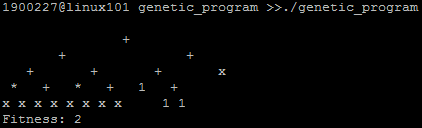
\includegraphics[width=0.75\textwidth]{gprun.png}
\end{center}
\caption{A Sample Genetic Program Run\label{fig:gprun}}
\end{figure}

